% !TEX root = ../fib_poly.tex

\begin{figure}[h!]
\centering
\resizebox{0.7\linewidth}{!}{
\begin{tikzpicture}[>=stealth]

\path[<-] (3.5,0)node[right]{$ $} edge(-1,0) (0,3)node[above]{$ $} edge(0,-1);

\node at(0,-0.01){$\bullet$};

\node at(-0.25,-0.25){$0$};

\node at(2,-0.01){$\bullet$};

\draw[thick] (0,0)--(2,0);

\node at(2.25,-0.25){$1$};

\end{tikzpicture}
\quad \resizebox{0.05\linewidth}{!}{\raisebox{3em}{$\longrightarrow$}} \quad \quad
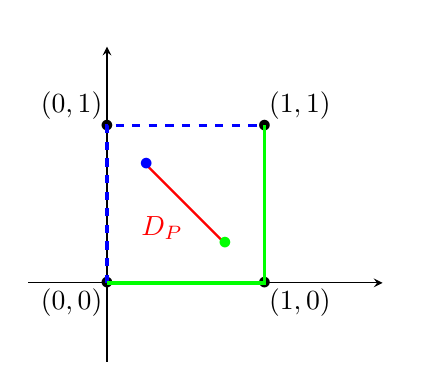
\begin{tikzpicture}[>=stealth]

\path[<-] (3.5,0)node[right]{$ $} edge(-1,0) (0,3)node[above]{$ $} edge(0,-1);

\node at(0,-0.01){$\bullet$};

\node at(-0.45,-0.25){$(0,0)$};

\node at(2,-0.01){$\bullet$};

\node at(2.45,-0.25){$(1,0)$};

\node at(2,2-0.01){$\bullet$};

\node at(2.45,2.25){$(1,1)$};

\node at(0,2-0.01){$\bullet$};

\node at(-0.45,2.25){$(0,1)$};

\draw[thick] (0,0)--(2,0)--(2,2);

\draw[thick, red] (0.25*2,0.75*2)--(0.75*2,0.25*2);

\node at(0.5,1.5){\color{blue}$\bullet$};

\node at(1.5,0.5){\color{green}$\bullet$};

\node at(0.7,0.7){\color{red}$D_P$};

\draw[very thick, blue,dashed] (0,0)--(0,2)--(2,2);
\draw[very thick, green] (0,0)--(2,0)--(2,2);

\end{tikzpicture}}
\caption{The polytope of diagonals of the interval (in red). Its two vertices define cellular approximations of the diagonal (dashed, in blue, and in green).}
\label{figure:cellularapproximation}
\end{figure}